We compare \sys\/ in HBase to the baseline MemStore implementation.  
Our evaluation explores all \sys\/ policies and configuration parameters.  
We experiment with two types of production machines with directly attached SSD 
and HDD storage. 

We study HBase throughput and latency, under a variety of workloads. 
To reason about the results, we explore additional signals -- I/O statistics, 
GC metrics, etc.  

We present the experiment setup in Section~\ref{ssec:setup}, and the evaluation 
results in Section~\ref{ssec:results}. 

\subsection{Experiment Setup}
\label{ssec:setup}

Our experiments exploit two clusters with different hardware types. The first cluster consists of five 12-core Intel Xeon 5 
machines with 48GB RAM and 3TB SSD storage. The second cluster consists of five 8-core Intel Xeon E5620 servers 
with 24GB RAM and 1TB HDD storage. Both clusters have a 1Gbps Ethernet interconnect. We denote these clusters 
SSD and HDD, respectively.

In each cluster, we use three nodes for HDFS and HBase instances, which share the hardware. The HDFS data 
replication ratio is 3x. HBase exploits two machines as region servers, and one as master server. 

A region server runs  with 8GB heap, configured with G1GC memory management. 
We use the default memory layout,  which allocates $40\%$ of the heap (roughly 3GB) to the MemStore 
area, and $40\%$ more to the read-path block cache. We apply an asynchronous WAL, to focus on real-time, 
write-intensive workloads (synchronous WAL implies an order-of-magnitude slower writes). The log aggregation
period is 1s. 
%The number of worker threads is 8, number of disk-flush threads is 10, and the maximal number 
%of HFile's per store is 25. 

The data resides in one table that is pre-split to 50 regions (i.e., each region server maintains 25 regions). 
The table has a single column family with four columns. 
%Our benchmarks build and query a dataset of 50-100 GB in each experiment. 

The workload is driven by the two remaining machines, each running up to 12 client threads. 
We use a popular YCSB benchmarking tool~\cite{Cooper:2010:BCS:1807128.1807152} to generate 
the put and get requests. All puts writes a full row (4 cells of 25 bytes each), and all gets retrieve
a single cell. Such small values are typical in production workloads~\cite{Wu2015}. 

In order to maximize the load, updates are batched at the client side in 10KB buffers. 
In each experiment, all operations draw keys from the same distribution over a key range
of 100M items. We experiment with two distributions: heavy-tailed (Zipf) and uniform (the latter 
is less representative of real workloads -- studied for reference only). The Zipf distribution 
is generated following the description in~\cite{Gray:1994:QGB:191839.191886}, with $\theta=0.99\%$ 
(YCSB standard).

\subsection{Evaluation Results}
\label{ssec:results}

We compare multiple \sys\/ policies (\basic, \eager, and \adp\/) to the legacy MemStore implementation,
(\none), which does not apply in-memory flush and compaction. \adp\/ is studied under multiple 
redundancy thresholds: $R=0.2$, $R=0.35$ and $R=0.5$ (the smaller the ratio, the more aggressively
the policy triggers in-memory compaction).  The $A$ (active segment bound) and $S$ (pipeline size bound) 
parameters are tuned for optimal performance. We use $A=0.02$ and $S=5$. Section~\ref{ssec:tuning} 
describes the exploration procedure. 

\subsubsection{Write-Only Workloads}

\begin{figure*}[tb]
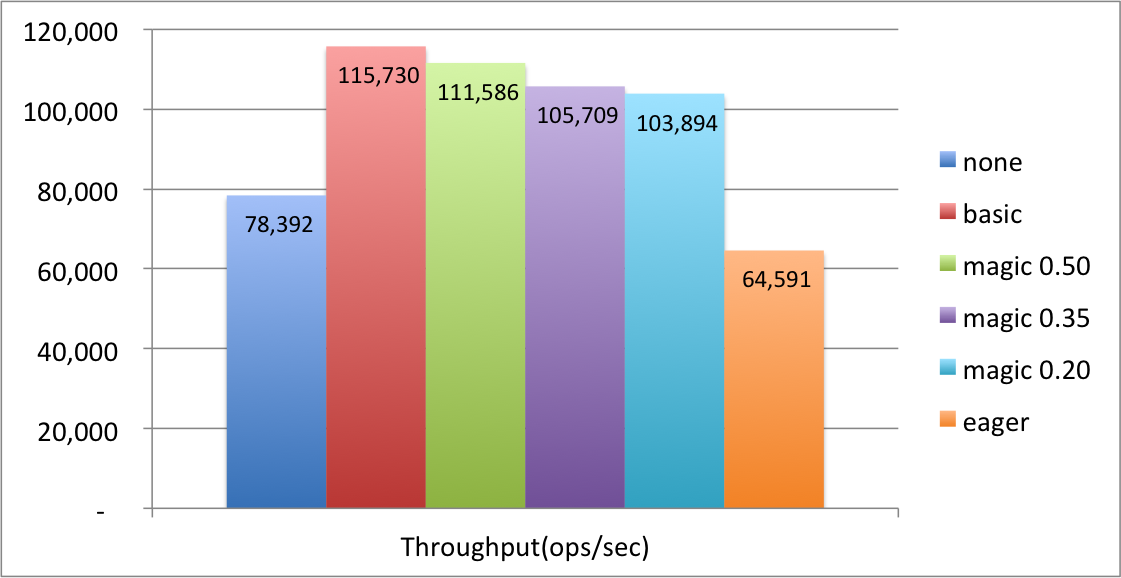
\includegraphics[width=\figw]{Figs/throughput-ssd.png}
\caption{{\bf  Throughput measured in SSD.} 
}
\label{fig:write-throughput}
\end{figure*}

The first experiment exercises only put operations. It starts from an empty table and performs 500M puts, 
in parallel from 12 client threads. We study the Zipf and the uniform key distributions.  

Figure~\ref{fig:write-throughput} depicts the throughput speedup for different policies and hardware types, 
and Table~\ref{tab:write-throughput} provides the absolute throughput numbers. For the Zipf benchmark, 
the maximal speedup are $47.6\%$ on SSD and $25.4\%$ on HDD. For the Uniform benchmark, they are 
$23.8\%$ and $8.9\%$, respectively. 

We see that the improvement is much higher for the system with SSD storage, which is much faster 
on the I/O side, and consequently overall. Being more CPU-bound than I/O-bound, its performance 
is heavily dependent on on the MemStore speed. By reducing the active segment size to only $2\%$
of the MemStore size, \sys\/ improves data locality and search time within the dynamic index. Moreover, 
it reduces by two orders of magnitude the number of small skiplist node objects, which relieves the 
pressure from the Java garbage collection. 

Somewhat surprisingly, the \eager\/ policy, albeit eliminating all redundant data, does not yield the largest 
throughput gain. We explain this by the overhead it incurs on the JVM by recycling the redundant cell 
objects at a very high rate. The \basic\/ policy, which releases large volumes of data at once upon disk 
flush, turns out to be more GC-friendly, and yields the best performance. Figure~\ref{fig:gc-throughput-log2}, 
which studies GC overhead for a range of policies and tuning parameters, further corroborates our 
hypothesis. We see a clear negative correlation between the GC cycles and the system performance. 

\begin{figure}[htb]
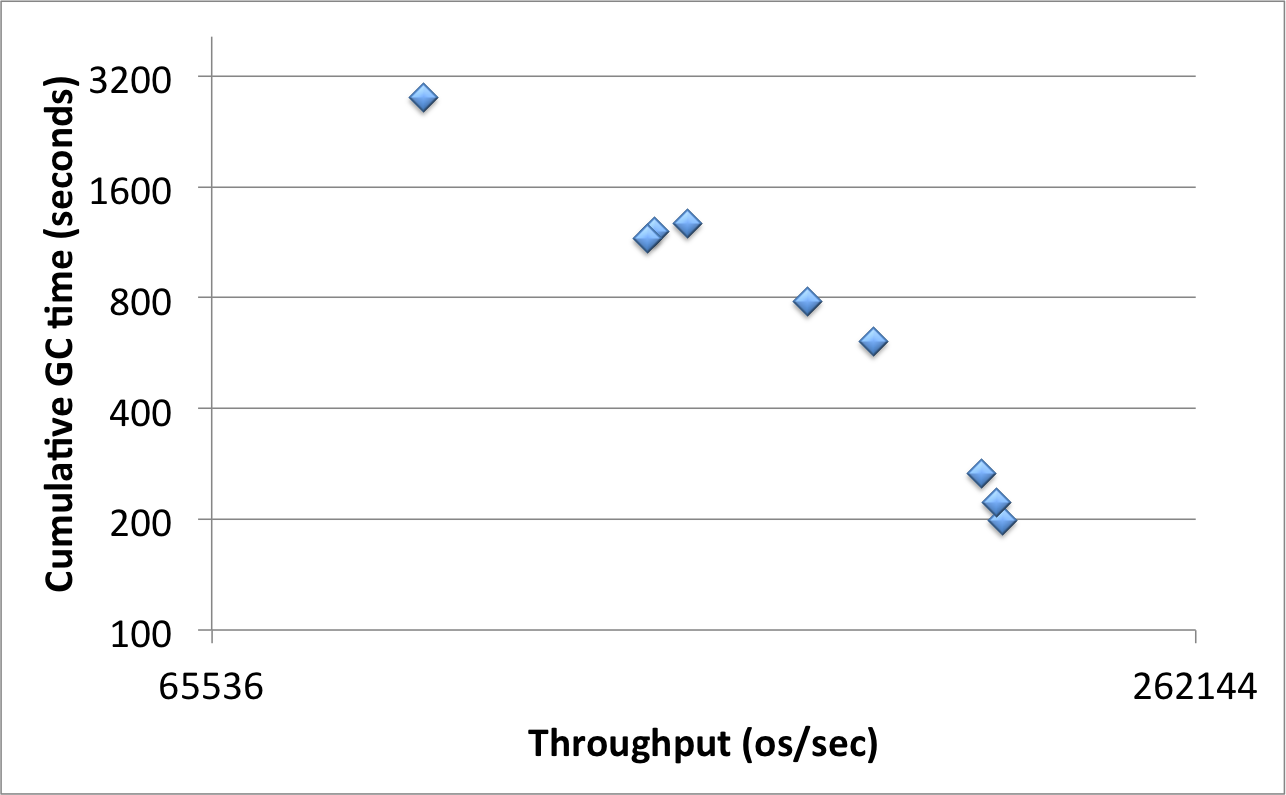
\includegraphics[width=\figw]{Figs/gc-throughput-log2.png}
\caption{{\bf GC-Throughput correlation.} Log-log scale plot of the cumulative gc time vs write throughput in different settings shows negative linear correlation.
}
\label{fig:gc-throughput-log2}
\end{figure}

\subsubsection{Read-Write Workloads}

\subsubsection{Parameter Tuning and Insights} \label{ssec:tuning}

 \remove{ 




We compare the strategies by measuring their throughput and latency. In addition we measure the write volume, that is the number of KB written to the file system, and the cumulative gc time of each run.

The results of the following experiments are presented:
(1) demonstrating the insight from different sets of experiments showing that gc overhead is a great throughput predictor,
(2) write-only workload - comparing all 4 strategies,
(3) mixed read-write workload - showing reduction in read latencies of \basic\ and \magic\ strategies with respect to \none.
(4) evaluating different settings of the \basic\ strategy in order to find its optimal configuration,

\paragraph{GC overhead.}

Our experiments show that in write-only workloads gc and throughput have a very high correlation. 
Figure~\ref{fig:gc-throughput-log2} plots the scatter graph of cumulative gc time vs write throughput of several write-only experiments with varying settings in different strategies. It clearly shows that  the lower the gc overhead is, the higher the throughput is.
Specifically, there is a negative linear correlation between their values on a log-log scale.




\paragraph{Write-only workload.}
Each run creates an empty 50 regions table and then utilizes 12 threads to run 500 million update operations, each writing to all columns. Each such run is repeated 5 times. 
We measure total  throughput and total volume of MB written to files. We present here the performance results of the run with the median throughput among 5 runs.

Figures~\ref{fig:throughput-ssd} and~\ref{fig:throughput-hdd} depict the lift in throughput \basic, \magic, and \eager\ achieve over \none in ssd and hdd, respectively.
Tables~\ref{fig:counters:ssd} and ~\ref{fig:counters:hdd} present the number of flushes, disk compactions and WAL files generated during the experiment.
Figures~\ref{fig:volume-ssd} and~\ref{fig:volume-hdd} depict the write volume in every setting. 
\magic demonstrates the tradeoff between throughput and write volume. As we increase the compaction threshold more in-memory compaction are triggered which degrades the throughput but at the same time reduces the write volume.
At the extremes are \basic\ with the highest throughput and \eager with lowest write volume.
\basic\ and \magic\ both run with $2\%$ active segment. In SSD the limit on the size of the pipeline is 5 and in HDD it is 4.
\eager\ runs with $25\%$ active segments and limit of 2 on the size of the pipeline.
The uniques thresholds for \magic\ are $0.2$, $0.35$, and $0.5$.



\begin{figure}[htb]
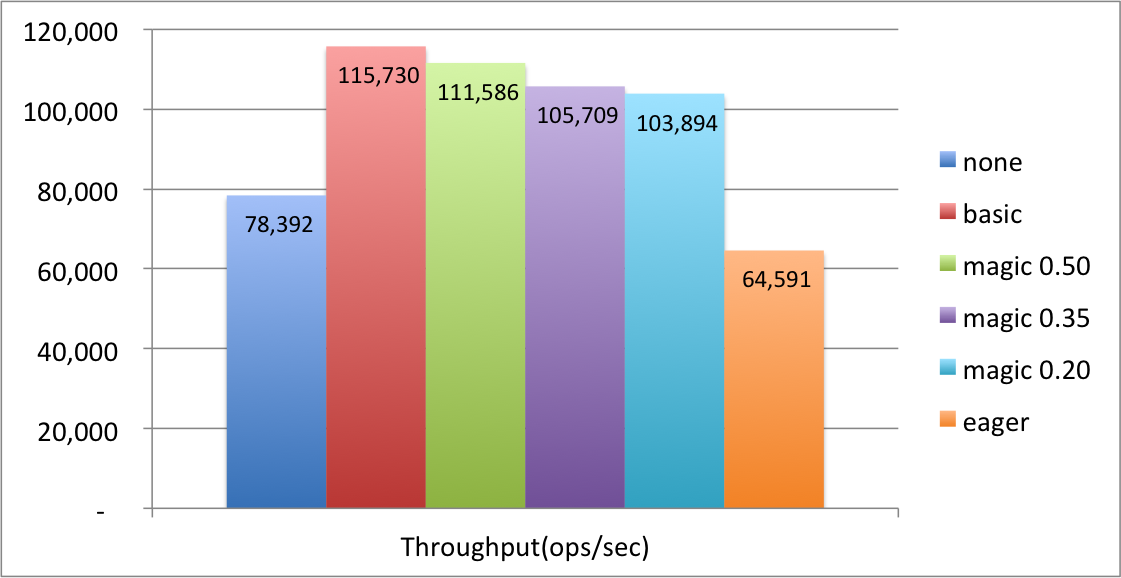
\includegraphics[width=\figw]{Figs/throughput-ssd.png}
\caption{{\bf  Throughput measured in SSD.} Zipfian distribution.
}
\label{fig:throughput-ssd}
\end{figure}

\begin{figure}[htb]
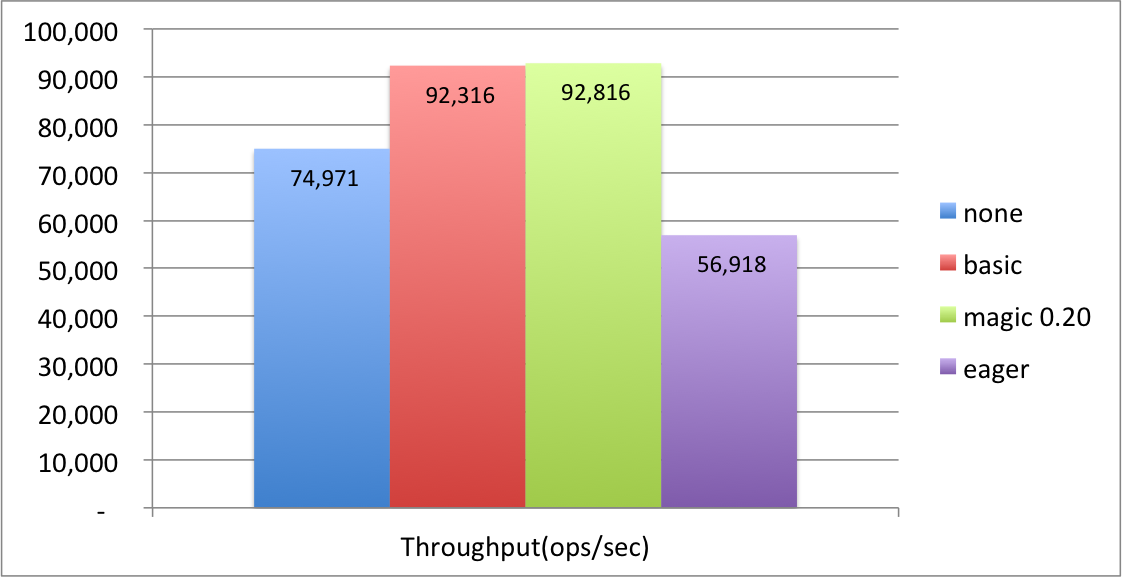
\includegraphics[width=\figw]{Figs/throughput-hdd.png}
\caption{{\bf  Throughput measured in HDD.} Zipfian distribution. 
}
\label{fig:throughput-hdd}
\end{figure}


\begin{figure}[!t]
  \centering
  
  \begin{subfigure}[tb]{\columnwidth}
      \centering\small
    \begin{tabular}{|c|c|c|c|}
      \hline
      Strategy & $\#$flushes & $\#$compactions & $\#$WAL files\\
      %\hline
      \hline
      \none & 1468	&524&	789 \\
\basic & 1224&	355&	806 \\
\magic\ 0.50 &922&	309&	678 \\
\magic\ 0.35 & 754&	261&	615 \\
\magic\ 0.20 & 631	&209	&533 \\
\eager\ & 695	&242&	490 \\
      \hline
    \end{tabular}
	\caption[]{SSD}
    \label{fig:counters:ssd}
  \end{subfigure}
  
  \begin{subfigure}[t]{\columnwidth}
    \centering\small
    \begin{tabular}{|c|c|c|c|c|}
      \hline
        Strategy & $\#$flushes & $\#$compactions & $\#$WAL files\\
      %\hline
      \hline
      \none & 1504 & 548 & 743 \\
\basic & 1210 & 443 & 808 \\
\magic\ 0.50 & 879 & 316 & 695 \\
\magic\ 0.35 & 711 & 248 & 650 \\
\magic\ 0.20 & 630 & 216 & 556 \\
\eager\ & 667 & 242 & 536 \\
      \hline
    \end{tabular}
	\caption[]{HDD}
    \label{fig:counters:hdd}
  \end{subfigure}


  \caption{Number of flushes, disk compactions, and WAL files created in different settings}
  \label{fig:counters}
\end{figure}


\begin{figure}[htb]
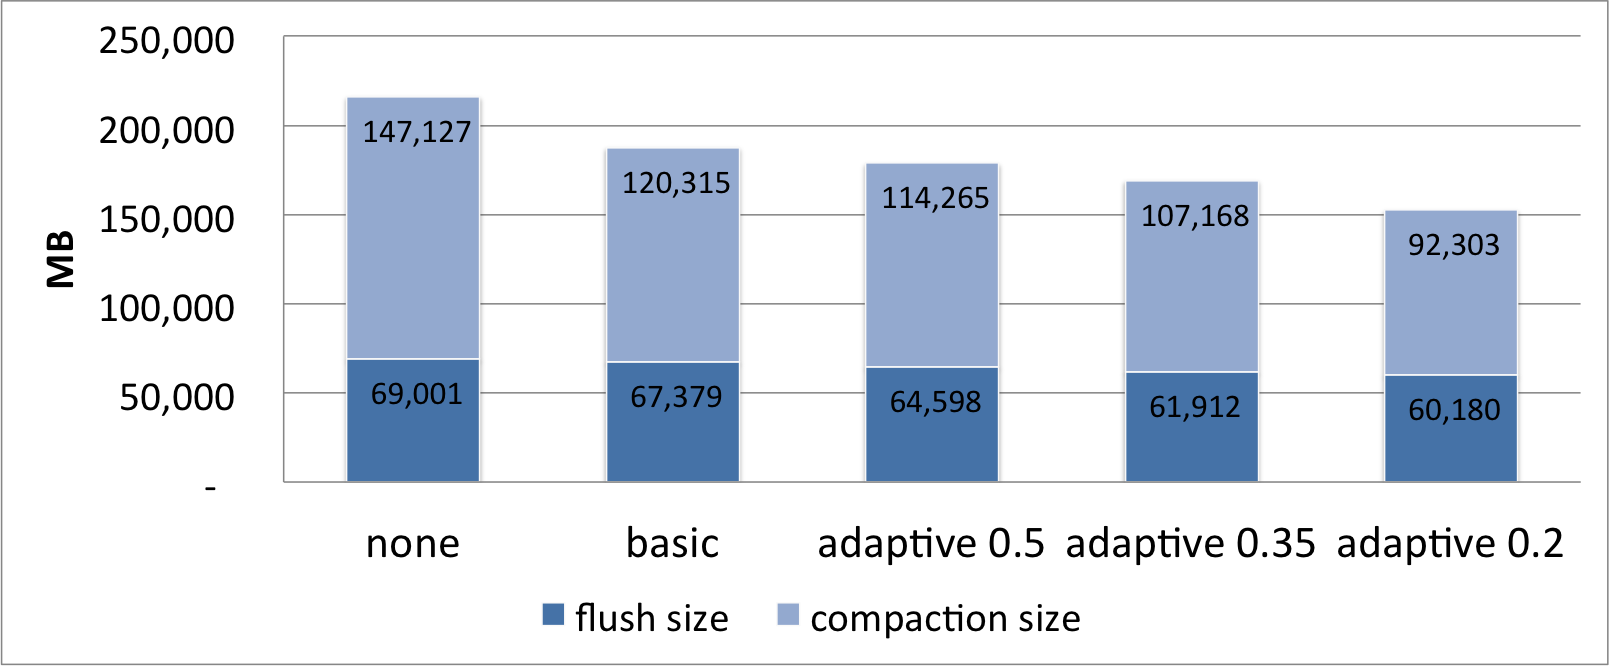
\includegraphics[width=\figw]{Figs/volume-ssd.png}
\caption{{\bf  Write volume in SSD.} Zipfian distribution.
}
\label{fig:volume-ssd}
\end{figure}

\begin{figure}[htb]
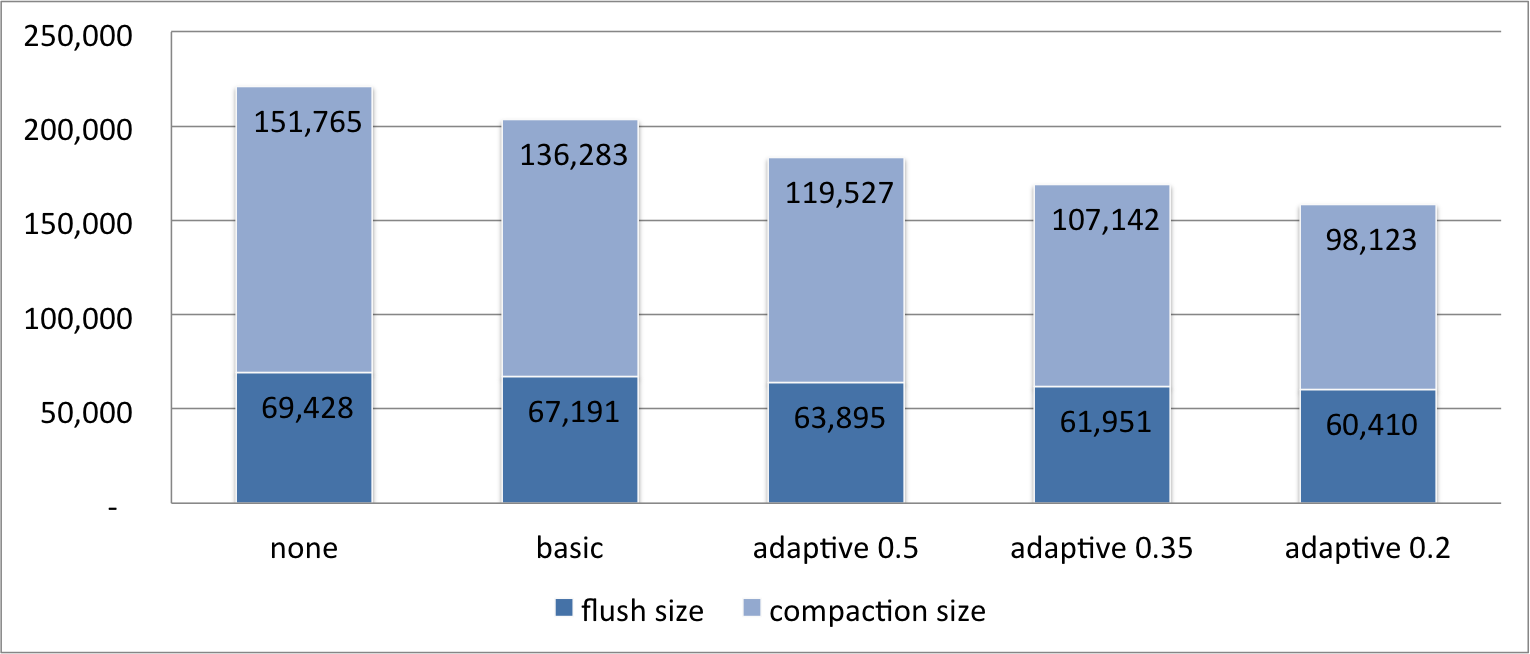
\includegraphics[width=\figw]{Figs/volume-hdd.png}
\caption{{\bf  Write volume in HDD.} Zipfian distribution.
}
\label{fig:volume-hdd}
\end{figure}

Figures~\ref{fig:throughput-ssd-uniform} and~\ref{fig:throughput-hdd-uniform} depict the throughput results with uniform distribution in ssd and hdd, respectively.
Tables~\ref{fig:counters-uniform:ssd} and ~\ref{fig:counters-uniform:hdd} present the number of flushes, disk compactions and WAL files generated during the experiment.
Figures~\ref{fig:volume-ssd-uniform} and~\ref{fig:volume-hdd-uniform} depict the write volume in every setting. 


\begin{figure}[htb]
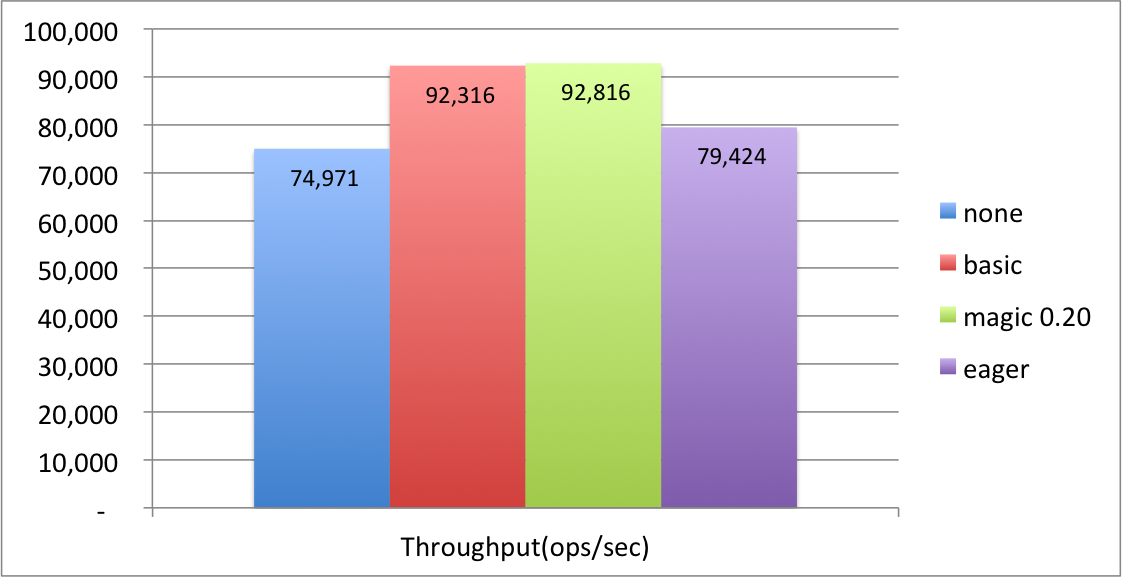
\includegraphics[width=\figw]{Figs/throughput-ssd-uniform.png}
\caption{{\bf  Throughput measured in SSD.} Uniform distribution.
}
\label{fig:throughput-ssd-uniform}
\end{figure}

\begin{figure}[htb]
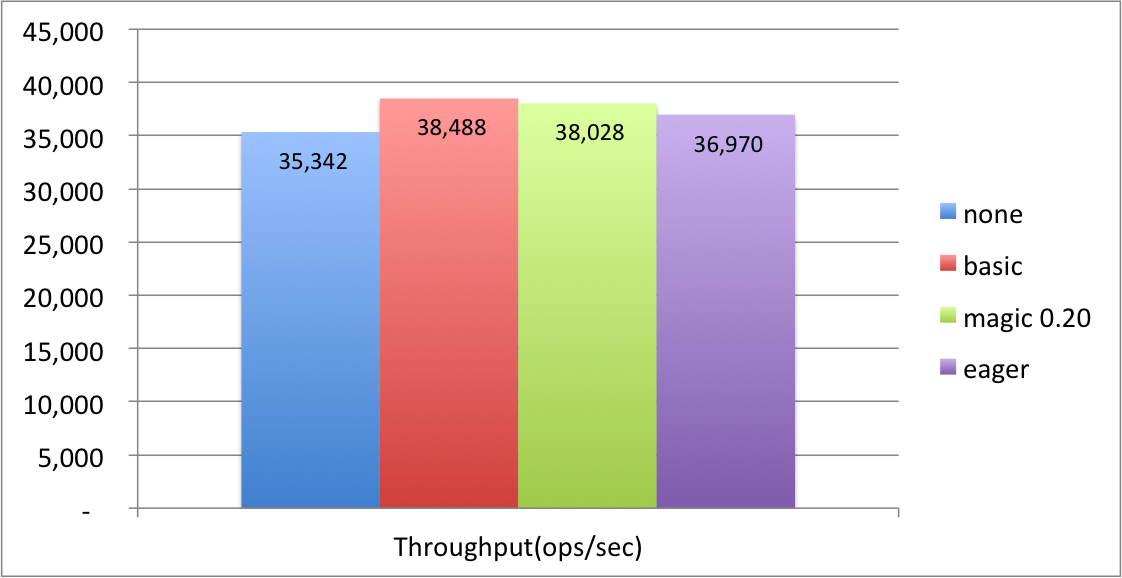
\includegraphics[width=\figw]{Figs/throughput-hdd-uniform.png}
\caption{{\bf  Throughput measured in HDD.} Uniform distribution. 
}
\label{fig:throughput-hdd-uniform}
\end{figure}


\begin{figure}[!t]
  \centering
  
  \begin{subfigure}[tb]{\columnwidth}
      \centering\small
    \begin{tabular}{|c|c|c|c|}
      \hline
      Strategy & $\#$flushes & $\#$compactions & $\#$WAL files\\
      %\hline
      \hline
\none & 1705 & 288 & 632 \\
\basic & 1416 & 220 & 577 \\
\magic\ 0.20 & 1402 & 219 & 586 \\
\eager\ & 1382 & 255 & 578 \\
       \hline
    \end{tabular}
	\caption[]{SSD}
    \label{fig:counters-uniform:ssd}
  \end{subfigure}
  
  \begin{subfigure}[t]{\columnwidth}
    \centering\small
    \begin{tabular}{|c|c|c|c|c|}
      \hline
        Strategy & $\#$flushes & $\#$compactions & $\#$WAL files\\
      %\hline
      \hline
     \none & 1736	&570&	739 \\
\basic & 1408&	458&	742 \\
\magic\ 0.20 & 1413	&470	&770 \\
\eager\ & 1423	&476&	760 \\
      \hline
    \end{tabular}
	\caption[]{HDD}
    \label{fig:counters-uniform:hdd}
  \end{subfigure}


  \caption{Number of flushes, disk compactions, and WAL files created in different settings with uniform distribution}
  \label{fig:counters-uniform}
\end{figure}


\begin{figure}[htb]
%\includegraphics[width=\figw]{Figs/volume-ssd-uniform.png}
\caption{{\bf  Write volume in SSD.} Zipfian distribution.
}
\label{fig:volume-ssd-uniform}
\end{figure}

\begin{figure}[htb]
%\includegraphics[width=\figw]{Figs/volume-hdd-uniform.png}
\caption{{\bf  Write volume in HDD.} Zipfian distribution.
}
\label{fig:volume-hdd-uniform}
\end{figure}



\paragraph{Mixed workload.}
Each run is comprised of two phases. 
The first phase creates an empty 50 regions table. It then loads the table with 10GB of data by running 100 million update operations chosen uniformly at random, each writing to all columns. 
The second phase measures the performance of a single thread running 150,000 read operation. 
We measure the 50-th, 75-th, 90-th, 95-th and 99-th percentiles.
An additional YCSB client is used to run background traffic. 
This client utilizes 12 threads to run update operations while we measure the read operations. 
Both reads and background traffic are chosen from a zipfian distribution.
Each such run is repeated 3 times. 

Figure~\ref{fig:latency-speedup-hdd} depicts the latency speed-up \basic\ and \magic\ achieve over \none.

\begin{figure}[htb]
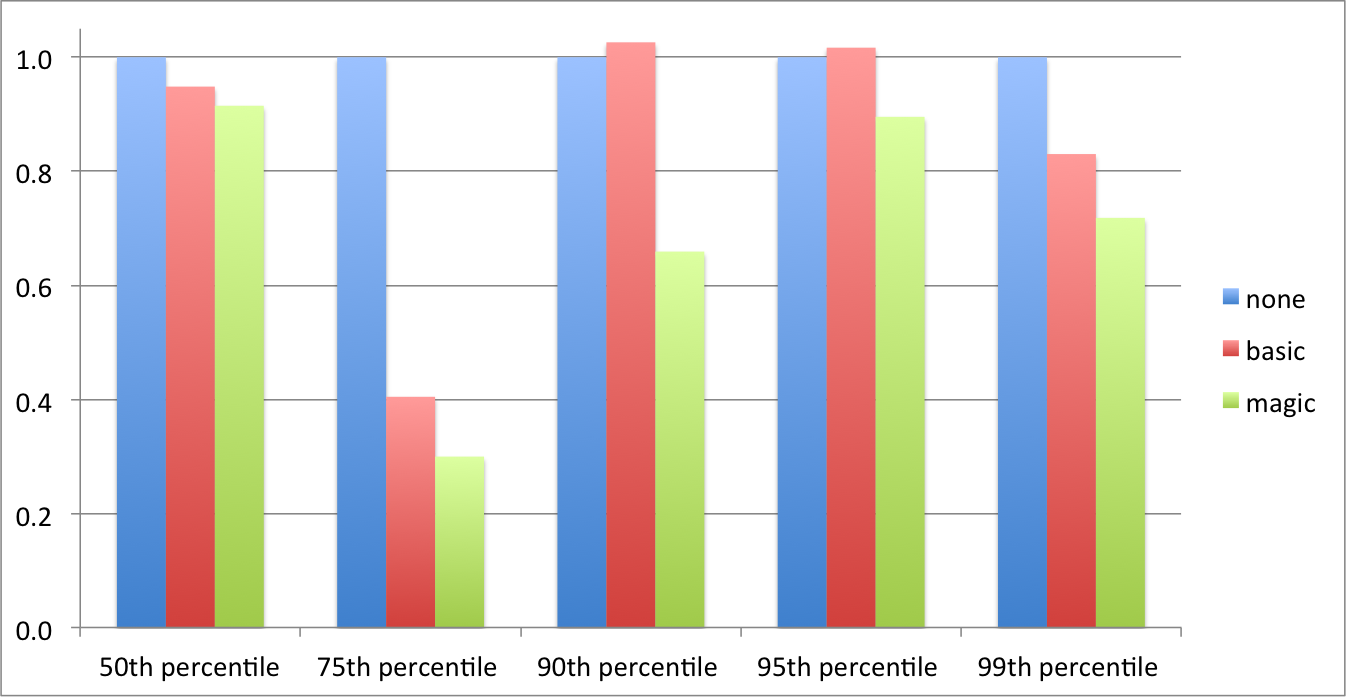
\includegraphics[width=\figw]{Figs/latency-speedup-hdd.png}
\caption{{\bf Latency speed-up in HDD.} 
}
\label{fig:latency-speedup-hdd}
\end{figure}

\paragraph{Parameter exploration.}
One of the main sources for memory management overhead is the skip-list data structure used to index the dynamic fraction of the memory component.
Not only it is bigger in size compared to a flat index it is also fragmented whereas static index is stored in a consecutive block of memory, therefore it incurs smaller overhead in terms of allocation, gc and cache misses.
We evaluate \basic\ strategy with different dynamic fraction sizes. We measure their throughput in write-only workload with zipfian distribution.
The throughput results of all runs are depicted in  Figure~\ref{fig:dynamic-fraction}. 
The \none\ strategy has no static portion in the memory component therefore its throughput is added at the point where the dynamic fraction size is equal to 1.0.
Figure~\ref{fig:dynamic-fraction} shows that indeed the store scales as the dynamic fraction size decreases. 

\begin{figure}[htb]
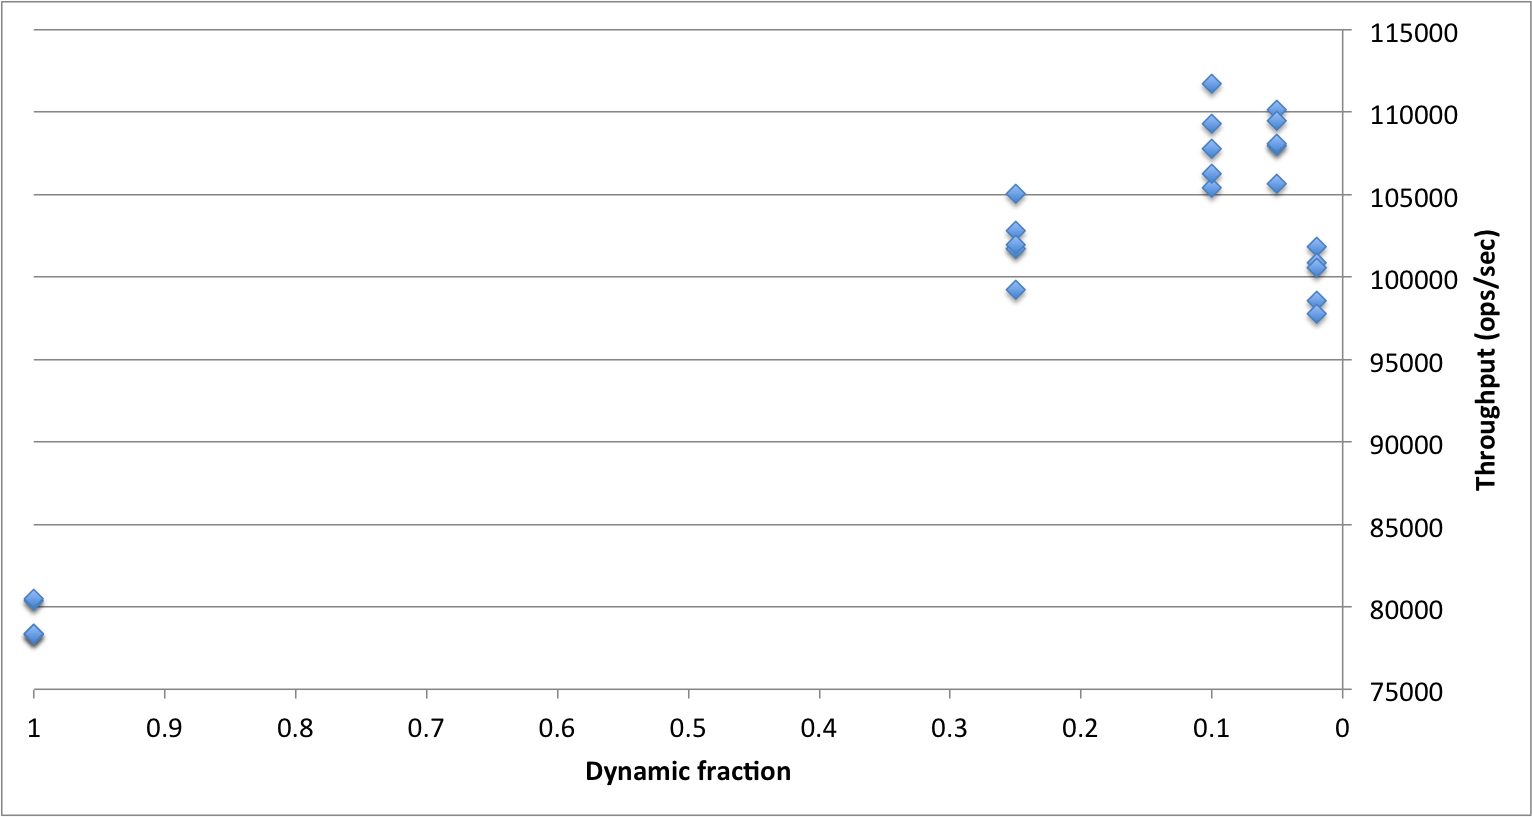
\includegraphics[width=\figw]{Figs/dynamic-fraction-1.png}
\caption{{\bf Dynamic fraction tuning.} The throughput increases as the dynamic fraction size decreases.
}
\label{fig:dynamic-fraction}
\end{figure}

When the dynamic fraction is less than $10\%$ it is clear that merging it into the much bigger static data over and over again can be inefficient as it creates a new index and dismisses the old one. 
The alternative is to enable several segments to wait in the pipeline before they are merged to a single segment. This helps with creating new index less frequently.
On the flip side, each segment in the pipeline calls for a separate scanner during read operations which can degrade their performance.
%Hence, we run the same experiments as explained above, varying the limit for the size of pipeline.
Figures~\ref{fig:pipeline-1-ssd} and~\ref{fig:pipeline-1-hdd} depict the throughput results as a function of the pipeline size. Peak throughput is with XX entries in the pipeline.

\begin{figure}[htb]
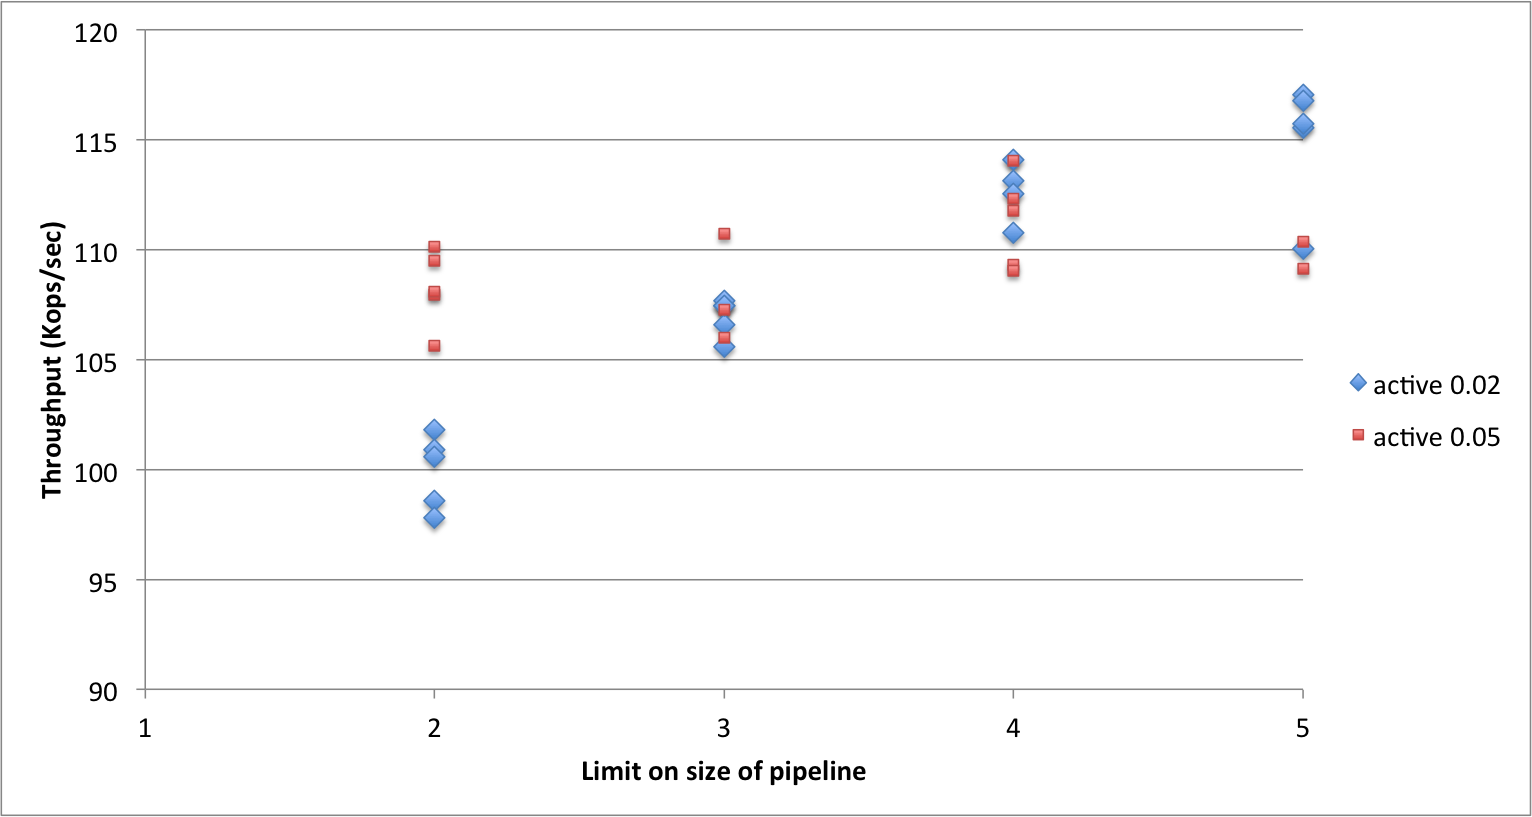
\includegraphics[width=\figw]{Figs/pipeline-1-ssd.png}
\caption{{\bf Pipeline size tuning - SSD.} 
}
\label{fig:pipeline-1-ssd}
\end{figure}

\begin{figure}[htb]
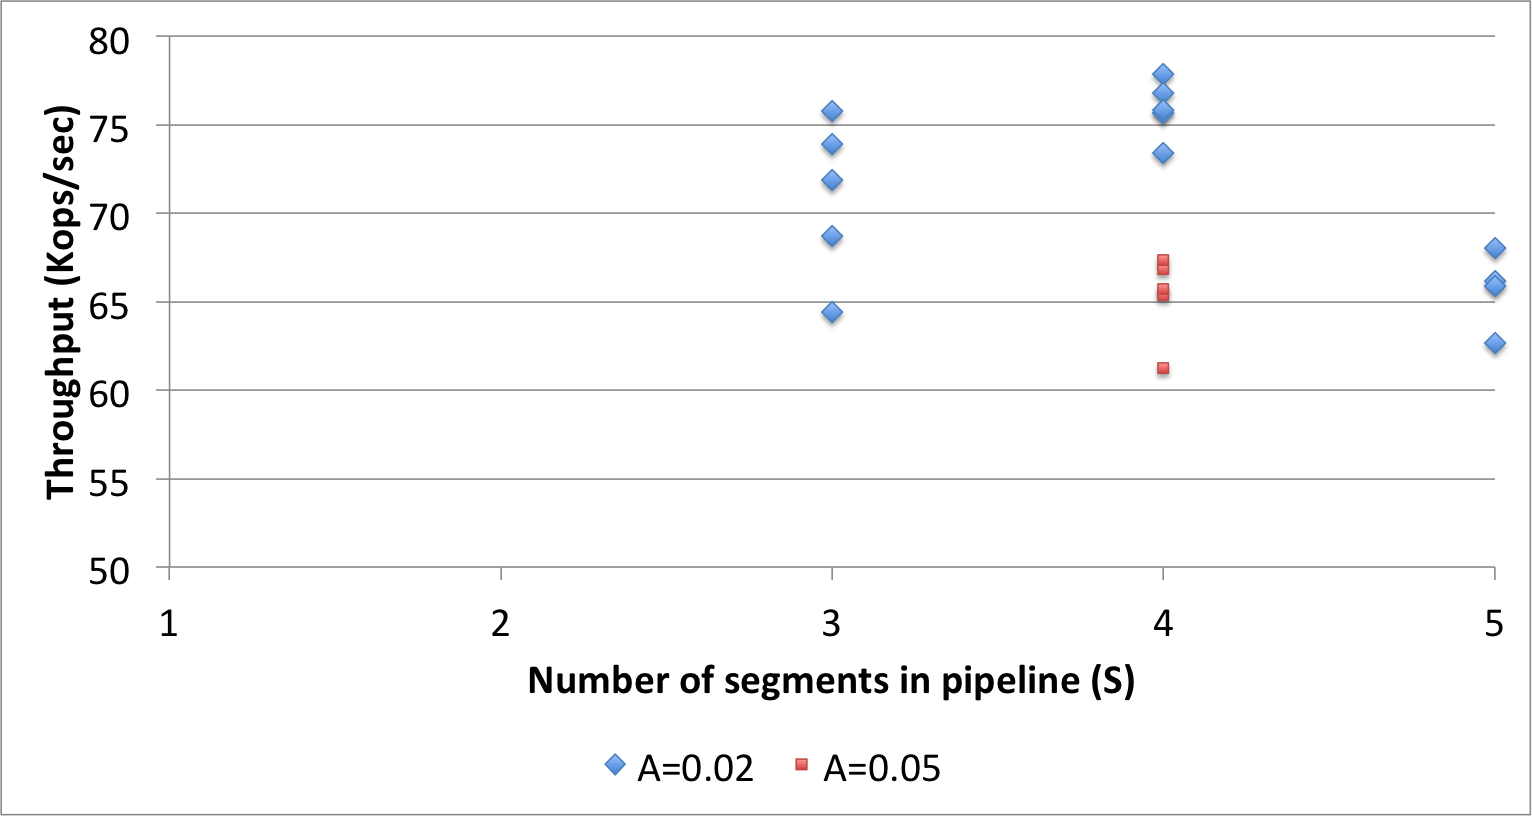
\includegraphics[width=\figw]{Figs/pipeline-1-hdd.png}
\caption{{\bf Pipeline size tuning - HDD.} 
}
\label{fig:pipeline-1-hdd}
\end{figure}

With a different experimental setup the tuning results are different.
For example when running similar workload with 100 regions and 16GB heap per region server we get different results.
\begin{figure}[htb]
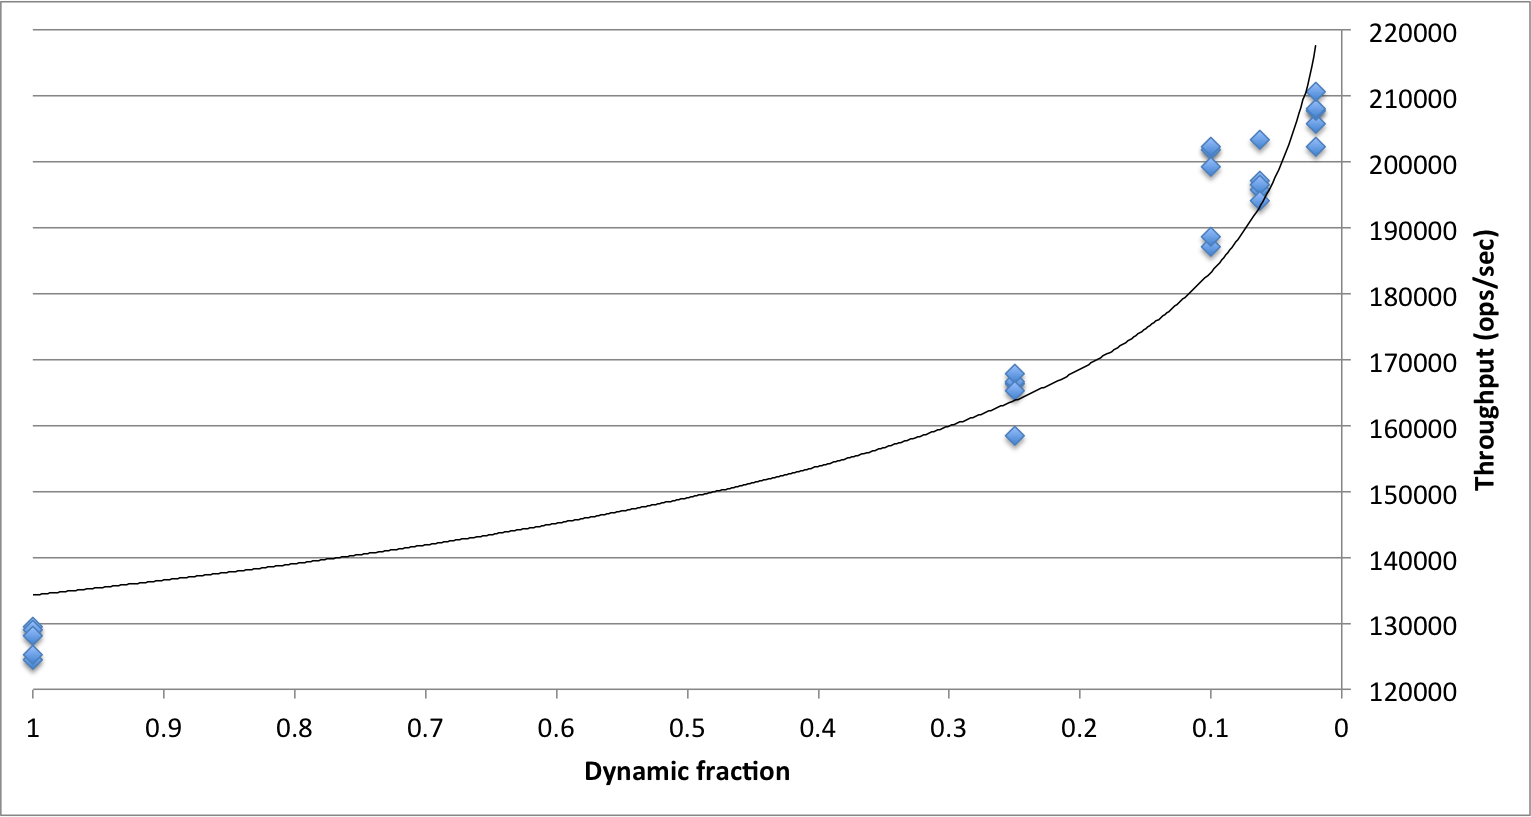
\includegraphics[width=\figw]{Figs/dynamic-fraction-2.png}
\caption{{\bf Dynamic fraction tuning.} 
}
\label{fig:dynamic-fraction-2}
\end{figure}

\begin{figure}[htb]
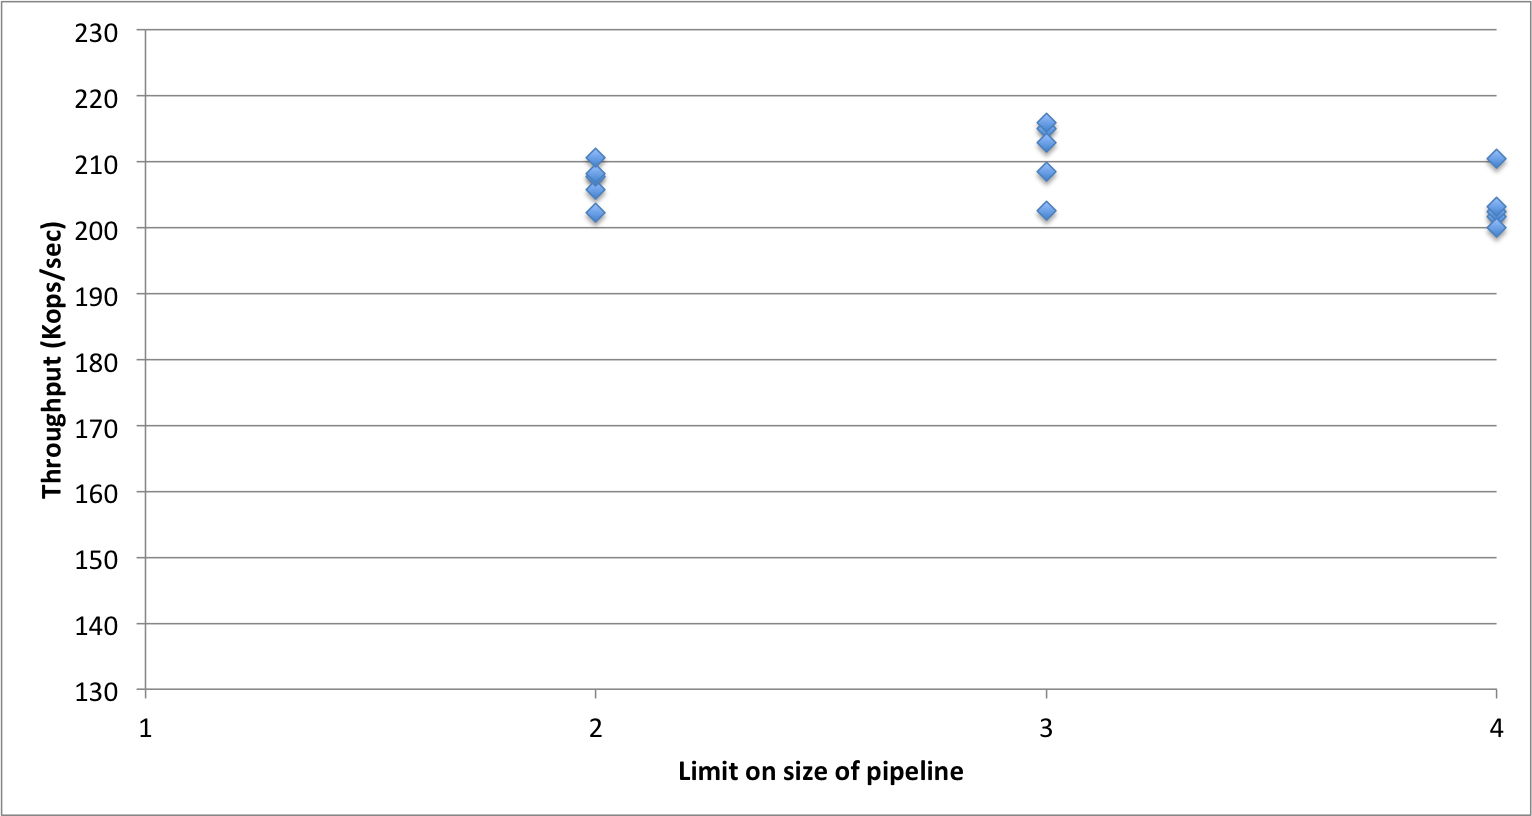
\includegraphics[width=\figw]{Figs/pipeline-2.png}
\caption{{\bf Pipeline size tuning.} 
}
\label{fig:pipeline-2}
\end{figure}

}